\documentclass{vldb}
\usepackage{times}
\usepackage{paralist}
% Load basic packages
\usepackage{balance}  % to better equalize the last page
\usepackage{graphicx} % for EPS, load graphicx instead
\usepackage{url}      % llt: nicely formatted URLs
\usepackage{amsmath}
\usepackage{color}
\usepackage{listings}
%\usepackage{wrapfig}
\usepackage{graphicx}
%\usepackage{subcaption}
\usepackage[english]{babel}
\usepackage{booktabs}
\usepackage{graphicx}
\usepackage{subfigure}
\usepackage{caption}
% \usepackage[scriptsize, it, IT]{subfigure}
% \usepackage[font={scriptsize,it}]{caption}
\usepackage{tikz}
%\usepackage{MinionPro}
\usetikzlibrary{arrows,matrix,positioning}
\usepackage[ruled,vlined,algonl,boxed]{algorithm2e}
\usepackage{framed}
\usepackage{enumitem}
\usepackage{xspace}
\usepackage{xcolor}
\usepackage{newtxmath}


% llt: Define a global style for URLs, rather that the default one
\makeatletter
\def\url@leostyle{%
  \@ifundefined{selectfont}{\def\UrlFont{\sf}}{\def\UrlFont{\small\bf\ttfamily}}}
\makeatother
\urlstyle{leo}

\makeatletter
\def\@copyrightspace{\relax}
\makeatother

% To make various LaTeX processors do the right thing with page size.
\def\pprw{8.5in}
\def\pprh{11in}
\special{papersize=\pprw,\pprh}
\setlength{\paperwidth}{\pprw}
\setlength{\paperheight}{\pprh}
\setlength{\pdfpagewidth}{\pprw}
\setlength{\pdfpageheight}{\pprh}
\newcommand{\papertext}[1]{#1}
\newcommand{\techreport}[1]{}

\newtheorem{definition}{Definition}[section]
\newtheorem{proposition}[definition]{Proposition}
\newtheorem{lemma}[definition]{Lemma}
\newtheorem{remark}[definition]{Remark}
\newtheorem{corollary}[definition]{Corollary}
\newtheorem{claim}[definition]{Claim}
\newtheorem{theorem}[definition]{Theorem}
\newtheorem{heuristic}[definition]{Heuristic}
\newtheorem{example}[definition]{Example}
%\newtheorem{proof}[definition]{Proof}
\newtheorem{dimension}{Dimension}
\newcounter{prob}
\newtheorem{problem}[prob]{Problem}
\newtheorem{conjecture}[definition]{Conjecture}
\newtheorem{reduction}[definition]{Reduction}
\newtheorem{property}[definition]{Property}
\newtheorem{axiom}[definition]{Axiom}

\tikzset{
    %Define standard arrow tip
    >=stealth',
    %Define style for boxes
    punkt/.style={
           rectangle,
           rounded corners,
           draw=black, very thick,
           text width=6.5em,
           minimum height=2em,
           text centered},
    % Define arrow style
    pil/.style={
           ->,
           thick,
           shorten <=2pt,
           shorten >=2pt,}
}


% \setitemize{noitemsep,topsep=0pt,parsep=0pt,partopsep=0pt}

% \def\compactify{\itemsep=0pt \topsep=0pt \partopsep=0pt \parsep=0pt}
% \let\latexusecounter=\usecounter
% \newenvironment{CompactItemize}
%   {\def\usecounter{\latexusecounter}
%    \begin{itemize}[noitemsep,topsep=0pt,parsep=0pt,partopsep=0pt,leftmargin=*]}
%   {\end{itemize}\let\usecounter=\latexusecounter}
% \newenvironment{CompactEnumerate}
%   {\def\usecounter{\compactify\latexusecounter}
%    \begin{enumerate}[leftmargin=*]}
%   {\end{enumerate}\let\usecounter=\latexusecounter}


%%%  What is this?  Use enumitem instead
% 
% \newcommand{\squishlist}{
%    \begin{list}{$\bullet$}
%     { \setlength{\itemsep}{0pt}
%       \setlength{\parsep}{2pt}
%       \setlength{\topsep}{6pt}
%       \setlength{\partopsep}{0pt}
%       \leftmargin=25pt
% \rightmargin=0pt
% \labelsep=5pt
% \labelwidth=10pt
% \itemindent=0pt
% \listparindent=0pt
% \itemsep=\parsep
%     }
% }
% \newcommand{\squishend}{\end{list}}
% 
% 
% \newcommand{\squishframe}{\vspace{-6pt}
% \begin{framed} 
% \vspace{-6pt}}
% 
% \newcommand{\frameend}{\vspace{-6pt}
% \end{framed}
% \vspace{-6pt}}


% create a shortcut to typeset table headings
\newcommand\tabhead[1]{\small\textbf{#1}}




% Make sure hyperref comes last of your loaded packages, 
% to give it a fighting chance of not being over-written, 
% since its job is to redefine many LaTeX commands.
\usepackage[pdftex]{hyperref}
\hypersetup{
  colorlinks=true,
  linkcolor=darkred,
  citecolor=darkgreen,
  urlcolor=darkblue
}
\usepackage{cleveref} % After hyperref, listings



% Avoid widows and orphans
\widowpenalty=500
\clubpenalty=500

% % Aggressive figure placement
% \renewcommand{\topfraction}{0.9}
% \renewcommand{\bottomfraction}{0.8}
% \setcounter{topnumber}{2}
% \setcounter{bottomnumber}{2}
% \setcounter{totalnumber}{4}
% \setcounter{dbltopnumber}{2}
% \renewcommand{\dbltopfraction}{0.9}
% \renewcommand{\textfraction}{0.07}
% \renewcommand{\floatpagefraction}{0.7}
% \renewcommand{\dblfloatpagefraction}{0.7}





\definecolor{light-gray}{gray}{0.95}
\definecolor{darkred}{rgb}{0.7,0.25,0.25}
\definecolor{darkgreen}{rgb}{0.15,0.55,0.15}
\definecolor{darkblue}{rgb}{0.1,0.1,0.5}
\definecolor{blue}{rgb}{0.19,0.58,1}

\newcommand{\red}[1]{\textcolor{red}{#1}}
\newcommand{\green}[1]{\textcolor{green}{#1}}
\newcommand{\blue}[1]{\textcolor{blue}{#1}}
\newcommand{\orange}[1]{\textcolor{orange}{#1}}
\newcommand{\darkred}[1]{\textcolor{darkred}{#1}}
\newcommand{\darkgreen}[1]{\textcolor{darkgreen}{#1}}
\newcommand{\darkblue}[1]{\textcolor{darkblue}{#1}}


\newcommand{\alex}[1]{\noindent{\textcolor{darkgreen}{Alexandra: #1}}}
\newcommand{\xlw}[1]{\noindent{\textcolor{blue}{Xiaolan: #1}}}
\newcommand{\ewu}[1]{\noindent{\textcolor{red}{EWu: #1}}}
\newcommand{\stitle}[1]{\vspace{0.5em}\noindent\textbf{#1}}
\newcommand{\calF}[0]{$\cal{F}$}
\newcommand{\codesize}{\fontsize{7}{8}}
\newcommand{\xxx}[1]{{\fontsize{13pt}{13pt}\selectfont\textcolor{red}{#1}}}
\newcommand{\ind}{\hspace{\algorithmicindent}}
\newcommand{\sys}{{\sc QueryFix}\xspace}
\newcommand{\gcost}{{\sc Greedy-Cost}\xspace}

\newcommand{\deprecate}[1]{\noindent{\color{light-gray}{#1}}}



% End of preamble. Here it comes the document.
\begin{document}

% for 
\title{Explaining Database Anomalies Via Queries}
%%
%% Title brainstorming
%%
%% Tracing data errors through query histories
%% Identifying query errors through data anomalies
%% Debugging query histories through data anomalies
%% Altering query histories to fix database anomalies
%% Query history manipulation: Indentifying query errors through data anomalies
%% Query-driven explanations to database anomalies

\numberofauthors{3}
\author{
  \alignauthor Xiaolan Wang\\
    \affaddr{School of Computer Science}\\
    \affaddr{University of Massachusetts}\\
    \email{xlwang@cs.umass.edu}\\
  \alignauthor Alexandra Meliou\\
  \affaddr{School of Computer Science}\\
    \affaddr{University of Massachusetts}\\
    \email{ameli@cs.umass.edu}\\
  \alignauthor Eugene Wu\\
    \affaddr{Computer Science}\\
    \affaddr{Columbia University}\\
    \email{eugenewu@mit.edu}\\
}



% Teaser figure can go here
%\teaser{
%  \centering
%  \includegraphics{Figure1}
%  \caption{Teaser Image}
%  \label{fig:teaser}
%}

\maketitle

\begin{abstract}
Data-driven applications rely on the correctness of their data to function
properly and effectively. Errors in data can be incredibly costly and
disruptive, leading to loss of revenue, incorrect conclusions, and misguided
policy decisions. While data cleaning tools can purge datasets of many errors
before the data is used, applications and users interacting with the data can
introduce new errors. Subsequent valid updates can obscure these errors and
propagate them through the dataset causing more discrepancies. Even when some
of these discrepancies are discovered, they are often corrected superficially,
on a case-by-case basis, further obscuring the true underlying cause, and
making detection of the remaining errors harder.

In this paper, we propose \sys, a framework that derives explanations for
discrepancies in datasets, by analyzing the effect of queries that operated on
the data and identifying potential mistakes in those queries. \sys is
flexible, handling scenarios where only a subset of the true discrepancies is
known, and robust, tolerating incorrectly identified discrepancies gracefully.
We make four important contributions: (a) we formalize the problem of
diagnosing the causes of data errors based on the queries that operated on the
dataset; (b) we develop exact methods for deriving diagnoses and fixes for
identified errors using state-of-the-art tools; (c) we present several
performance optimizations that scale diagnosis to large datasets and query
logs, while achieving near-optimal results; (d) we develop efficient
heuristics to gracefully handle mis-identified errors. We demonstrate the
effectiveness of \sys through extensive evaluation over real-world and
synthetic data.

\end{abstract}

%!TEX root=main.tex


%!TEX root = ../main.tex

\section{Introduction}
\label{s:intro}

\xxx{Sketch of arguments}

While exploring data, its natural to come across surprising or unexpected data.
For example, visual data analysis explores the current state of the database and users may be surprised by outliers in a visualization.
Similarly, enterprise customers (e.g., billing) may find outliers in their monthly bills and be surprised by the amount they are asked to pay.

When presented with these surprises, users want to better understand the reasons behind the anomalies.
A recent wave of research focuses on deriving predicate-based explanations for outliers for statistical aggregation queries.
For example, if the user wants to understand why the total sales in the past few months have gone up, these systems can general explanations such as ``most related to customers in California between the ages of 12 to 18.''
However, these approaches simply generate predicates that describe {\it current state} of the database, and do not resolve {\it how} the anomalous data came to be.

Specifically, the user may also be interested to understand which past database modification was responsible for these explanations.
Describe why this makes sense to want.  In this form of the problem, we are interested in historical database queries whose modifications, when propogated to the current database state, 
The goal is to provide diagnostic tools that can peer into past transactions.


In this paper, we approach anomaly explanation from the persepctive of the query log and seek to
both {\it identify}  historical database modification queries that most likely caused user complaints 
in the current state of the database, and suggest replacement queries that will resolve these complaints.
We call this problem the {\it Query-based Complaint-Satisfaction Problem}.

Given a database query log and a set of {\it complaints} (e.g., tuple 1's attribute B should be 20\% lower) about records in the current state of the database,
we seek to identify the subset of queries in the log that, by modifying their parameters and propogating the new effects of the queries, 
will best resolve the complaints.  

One way to solve this problem is to try modifying the most recent query until it fixes the complaints.  
If not, then try the second most recent query.  
The problem with this approach is the number of possible modifications is unbounded.

Our contributions include

\begin{enumerate}
\item Developing and formalizing the problem of Query-oriented explanation in contrast to data-oriented explanation
\item Prove that the general problem is impossible.
\item Designing alogirthems to solve the problem for complete complaint sets
\item Extending the algorithms to support incomplete complaint sets
\item Extending to support multiple queries
\end{enumerate}



\section{Use Case}

\section{Architecture}










%!TEX root = ../main.tex

\section{Modeling abstractions}
\label{sec:abstractions}

In this section, we introduce a running example inspired from the use-case of
Example~\ref{ex:taxes}, and describe the model abstractions that we use to
formalize the diagnosis problem.



%!TEX root = ../main.tex


\begin{figure*}[t]
    \begin{minipage}[t]{0.28\textwidth}
         \vspace{0pt} 
         \centering
        \begin{tabular}{llll}
            \multicolumn{4}{l}{\emph{Taxes}: $D_0$}\\
            \toprule
            \textbf{ID}  & \textbf{rate}  & \textbf{income}    & \textbf{owed}\\
            \midrule
            $t_1$   & 10    & \$9500    & \$950\\
            $t_2$   & 25    & \$90000   & \$22500\\
            $t_3$   & 25    & \$86000   & \$21500\\
            \bottomrule
            \\
        \end{tabular}
    \end{minipage}
    \begin{minipage}[t]{0.43\textwidth}
         \vspace{0pt} 
         \centering
        \begin{tabular}{|p{1ex}l|}
            \multicolumn{2}{l}{\emph{Query log}: $\mathcal{Q}$}\\
            % \toprule
            \hline
            $q_1$: & {\small UPDATE Taxes SET rate = 30}\\
                   & {\small WHERE income >= \color{red}{85700}} \\
            
            $q_2$: & {\small UPDATE Taxes SET owed = income*rate/100}\\
            
            $q_3$: & {\small INSERT INTO Taxes}\\ &{\small VALUES (4, 25, 86500, 21625)}\\
            \hline
            % \bottomrule
        \end{tabular}
    \end{minipage}
    \begin{minipage}[t]{0.28\textwidth}
         \vspace{0pt} 
         \centering
        \begin{tabular}{llll}
            \multicolumn{4}{l}{\emph{Taxes}: $D_3$}\\
            \toprule
            \textbf{ID}  & \textbf{rate}  & \textbf{income}    & \textbf{owed}\\
            \midrule
            $t_1$   & 10    & \$9500    & \$950\\
            $t_2$   & 30    & \$90000   & \$27000\\
            \rowcolor{mid-gray}
            $t_3$   & \color{red}{30}    & \$86000   & \color{red}{\$25800}\\
            $t_4$   & 25    & \$86500   & \$21625\\
            \bottomrule
        \end{tabular}
    \end{minipage}

    \caption{A recent change in tax rate brackets calls for a tax rate of 30\% for those with income above \$87500.  The accounting department issues query $q_1$ to implement the new policy, but the predicate of the WHERE clause condition transposed two digits of the income value.  As a result, the tax rate of $t_3$ was increased incorrectly.  Query $q_2$ that calculates the amount owed based on the corresponding tax rate and income propagates the error.  The mistake is further obscured by query $q_3$, which inserts a tuple with similar income and the correct tax rate.}
    \label{fig:example}
\end{figure*}

\begin{example}\label{ex:taxes2}
    
Figure~\ref{fig:example} demonstrates an example tax bracket adjustment in the
spirit of Example~\ref{ex:taxes}. The adjustment sets the tax rate to 30\% for
income levels above \$87,500, and is implemented by query $q_1$. A digit
transposition mistake in the query, results in an incorrect tax rate for tuple
$t_3$. Query $q_2$ that calculates the amount owed based on the corresponding
tax rate and income propagates the error to other fields. The mistake is
further obscured by query $q_3$, which inserts a tuple with slightly higher
income than $t_3$ and the correct (lower) tax rate.

\end{example}
% 
While traditional data cleaning techniques seek to identify and correct the
erroneous values in the table \emph{Taxes} directly, our goal is to diagnose
the problem, and understand the reasons for these errors. In this case, the
reason for the data errors is the incorrect predicate value in query $q_1$.

In this paper, we assume that we know \emph{some} errors in the dataset, and
that these errors were caused by erroneous updates. The errors may be
obtained in different ways: traditional data cleaning tools may identify
discrepancies in the data (e.g., a tuple with lower income has higher tax
rate), or errors can be reported directly from users (e.g., customers
reporting discrepancies to customer service). \emph{Our goal is not to correct
the errors directly, but to analyze them as a ``symptom'' and provide a
diagnosis.} The diagnosis can produce a targeted treatment: knowing how the
errors were introduced guides the proper way to trace and resolve them.


%!TEX root=../main.tex

\begin{figure}[t]
\centering
{\small
\begin{tabular}{ll}
    \toprule
    \textbf{Notation} & \textbf{Description}\\
    \midrule
    $D_0$    & Initial database state at beginning of log\\
    $\mathcal{Q}$& The sequence of executed update queries (log)\\ 
             & $\mathcal{Q}=\{q_1, \dots, q_n\}$ \\
    $D_n$    & End database state (current) $D_n=\mathcal{Q}(D_0)$\\
    $\mathcal{C}$ & Set of complaints $\mathcal{C}=\{c_1,\dots,c_k\}$\\
    $\mathcal{Q}^*$& Corrected query sequence \\
    \bottomrule
\end{tabular}
}
\caption{Summary of notations used in the paper.}
\label{tbl:notation}
\end{figure}

\subsection{The complaint provenance model}
\label{sec:model}

In our setting, the diagnoses are associated with errors in the queries that
operated on the data. In Example~\ref{ex:taxes2}, the errors in the dataset
are due to the digit transposition mistake in the WHERE clause predicate of
query $q_1$.  Our goal is to infer the errors in a log of queries automatically, given a set of incorrect values in the data.



\xxx{===}

First, some notation used in the rest of the paper.

Our goal is to take the user's complaints about the current state
of the database, and identify transformations over the database
query log that, when applied to the database, ``fixes'' these
complaints.  Although the general formulation of the problem that
we will introduce is intractable, we will reduce the scope of the
problem to a useful and tractable version.  To begin, we will
introduce the notation that is used in the rest of the paper.

\stitle{Def 1 (Database, State, Query)}: Let a database
be defined as the result of applying a sequence of queries in the query log
$Q_{seq}=\{Q_1,..., Q_n\}$ to an initial database $D_0$.  
Applying the query log to the initial database 
results in $n$ intermediate database states $\{D_i = Q_i(D_{i-1}) | i \in [1, n]\}$.  
where $D_n = Q_{seq}(D_0) = Q_n(\ldots Q_1(D_0))$ is the current state of the database. 
We assume that a subset of the query log has been replaced with {\it corrupted queries} 
such that $D_n$ and $Q_{seq}$ differ from the true database state $D^*_n$ and query log $Q^*_{seq}$.

In our current problem, we only deal with non aggregation and non-join queries.
In addition, for ease of exposition, we assume that the database contains a single table $T$ 
($T^*$ in the true database) containing $m$ numerical attributes $a_1,\ldots,a_m$, 
where the primary key is $a_1$.  
In Section~\ref{blah}, we will describe how our techniques extend to multi-table databases.
\xxx{Define the scope of queries supported}



\stitle{Def 2 (Complaints and Complaint Sets)}:
The tuple-wise difference between two databases $D_1$ and $D_2$ can be viewed as a patch
$P_{D_1, D_2}$ that contains {\it difference pairs} $(t_i \in T, t^*_i \in T^*)$.
Similar to source code patches, patches can be applied to a database $P(D_n) = D^*_n$.
Each pair in a patch describes one of three error types that can be present in $D_n$:

\begin{itemize}
\item {\it ADD}: $t^*_i$ should be added to the database $(\textrm{null}, t^*_i)$
\item {\it DELETE}: $t_i$ should be removed from the database $(t_i, \textrm{null})$
\item {\it WRONG}: $t_i$ should be modified into $t^*_i$
\end{itemize}


The user provides a {\it complaint set} $C$ that specify the perceived incorrect tuples in $D_n$.
$C$ is simply a patch.
We define a complete complaint set when $C = P_{D_n, D^*_n}$.
In contrast, an {\it incomplete complaint set}  may contain complaints that are false negatives (insertions that should be in $C$ but are not),
false positives (deletions that are not present), and errors (proposed value of a $t'$ is incorrect).

The accuracy of an incomplete complaint set can be measured by the ratio $acc_C = \frac{|C \cap \Delta|}{|\Delta|}$.



\begin{figure}[t]
\centering
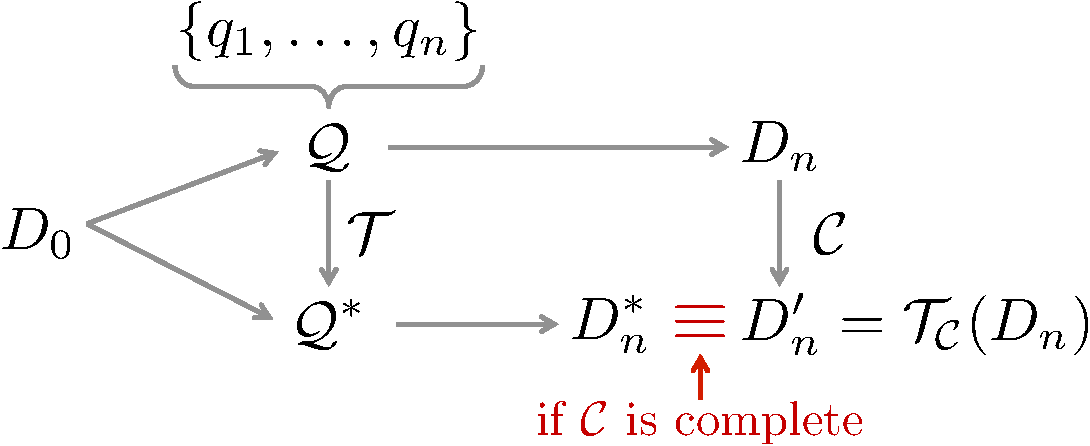
\includegraphics[width = 2in]{figures/probtransform}
\caption{Graphical depiction of the general \sys problem.}
\label{f:probtransform} 
\end{figure}



\subsection{Naive Formulation}

The most general version of the problem
(depicted in Figure~\ref{f:probtransform}) is to find a sequence of
transformations $T$ that insert, delete, and/or modify queries in $Q_{seq}$ 
such that the resulting sequence, $Q'_{seq} = T(Q_{seq})$, resolves the user's complaint set. 

However this problem is ill-defined because there exist an unbounded set of transformations that
can resolve the user's complaint set.  A naive solution is to append to the query log a statement
that deletes all the records in the database, followed by a query that insert all of the correct records.
Unfortunately this naive solution does not help explain the complaints in any way!

\subsection{Constraints}

For this reason, we constrain the set of possible transformations $\mathcal{T}$ to the following:

\begin{itemize}
\item delete query
\item modify insert statement constants
\item modify constants in WHERE clause
\end{itemize}

Our transformations don't include adding new queries, synthesizing arbitrary queries, or modifying the
number of clauses in a WHERE condition.  We apply these restrictions because we believe it is more likely
for the user to mis-type a constant value as opposed to having an error in the query structure.

Futhermore we define a distance metric between two query logs in order to evaluate
the qulatiy of a transformation.
\xxx{define $\mathcal{T}$ here.}



\subsection{Problem Statements}

In this paper, we present three variants of this problem.

\begin{problem}[Prob-Complete]\label{prob:complete}
Given $C = P_{D_n, D^*_n}$, $Q_{seq}$, and the sequence of database states $D_0,\ldots,D_n$, 
identify a sequence of transformations $T$ such that:
\begin{itemize}
\item $T(Q_{seq})(D_0) = C(D_n)$
\item $|T| = 1$
\item $T$ metric is minimized
\end{itemize}
\end{problem}

This variation of the problme relaxes the constraint that the complaint set must be complete, and allows
for both false positives as well as false negatives.  The goal is the same, however the constraints are relaxed:

\begin{problem}[Prob-Incomplete]\label{prob:incomplete}
Given $C$ where $acc_C < 1$, $Q_{seq}$, and the sequence of database states $D_0,\ldots,D_n$, 
identify a sequence of transformations $T$ such that:
\begin{itemize}
\item $T(Q_{seq})(D_0) = D^*_n$
\item $T$ metric is minimized.
\item $|T| = 1$
\end{itemize}
\end{problem}

Finally, we extend the problem to allow transformations with one or more operations.

\begin{problem}[Prob-MultiQ]\label{prob:multi}
Given $C$ where $acc_C < 1$, $Q_{seq}$, and the sequence of database states $D_0,\ldots,D_n$, 
identify a sequence of transformations $T$ such that:
\begin{itemize}
\item $T(Q_{seq})(D_0) = D^*_n$
\item $T$ metric is minimized.
\end{itemize}
\end{problem}




\subsection{A Naive Approach}

\begin{itemize}
\item roll back complaints to penultimate state using algebraic expressions 
\item perturb each expression in query until the query result matches correct state
\item if an expression cannot be found, iterate
\end{itemize}


Not clear how to roll back complaints

Ways to perturb query expressions is unbounded


\section{Basic Solution}

In this section we will introduce a simple approach to solve Prob-Complete.


Given $D^'_n = C(D_n)$, able to roll back to fixed intermediate state $D^'_i$.


\subsection{Metrics}

Metrics we use to measure how good a fix is.

Used in the optimization problem.




\subsection{Single-Query Case}

In this section, we walk through the core techniques in the case of a query sequence containing a single query.
\xxx{Walk through solution for each error type for each query type.}

Inserts and deletes are straight forward, however modifying WHERE clause is harder because
\xxx{why?}.  To deal with this challenge, we tried three algorithmic approaches.

\stitle{Constraint-solver (CPLEX)}
Describe how to encode problem as CPLEX

\stitle{Bounding Box}


\stitle{Decision Tree}
Describe how to encode as decision tree, what algorithm, and how to interpret learned tree.

Also, how to encode constraint that structure needs to be the same, by simply limiting the possible attribute
choices at each step in the learning algorithm.

\subsubsection{Comparing these approaches}

To understand the tradeoffs between these approachse, we ran a simple experiment for a single query.

Here are the results.


CPLEX takes the longest, however produces exact results.  However, it fails to produce any results if there are conflicting complaints.
Decision tree is fastest, however the quality of the results are poor.
Bounding box is similar to CPLEX in quality, however it generates results even if there are conflicting complaints.








\section{Prob-Complete}

Given the above, the algorithm for solving the complete complaint set problem is straightforward (Algorithm~\ref{alg:basic}).
We can simply try each query and return the one for which the best solution is found.

\subsection{Provenance-based Log Filtering}

Use provenance information (tuple-level or query level) to filter out queries that do not 
affect the complaint tuples at all.





\section{Incomplete Complaints}
\label{s:incomplete-algs}

Incomplete complaints are a challenge because the exesting algorithms fail.  We ran a simple experiment
where the complaint set contains only M\% of the true complaint set, and has N randomly generated erroneous complaints.
Figure~\ref{} shows that none of the algorithms work.

Describe assumptions for why a cleaning-based approach makes sense.

We use a cleaning-based method to deal with false positives, and some magic to deal with false negatives.

\subsection{False Positives}

Describe density, bi-partite graph, consistency, tuples affected scores.  Which ones work well, which ones don't.

NP-completeness of density-based approach.


\subsection{False Negatives}



\section{Multi-query Resolution}

We use a dynamic programming-based algorithm to support multiple queries.




\section{Rolling back the log}

Describe Alexandra's solver.

Algorithm:

\begin{verbatim}

querylog = filter(querylog)
batchsize = 1
while i > 0
  batch = [qi to q{i-batchsize}]
  alexandras_solver(batch)
  i -= batchsize

\end{verbatim}

\section{Implementation}

\sys is implemented as a Java-based middleware in front of PostgreSQL.

Talk about tricks to encode problem intto CPLEX/decision tree?



\section{Experiments}

We have two goals for our evaluation: First, we study how effectively
the techniques proposed in this paper are able to identify and fix
a single corrupt query in various types of query logs.  Second, we
seek to understand the conditions in which our multi-query techniques
are effective.  Finally, we want to understand how different
parameters of our roll-back technique affects the quality of our
proposed fixes.

To this end,
we ran a combination of synthetically generated query logs, and
well as logs generated using a subset of the TPC-C~\cite{tpcc}
transaction log that consists of inserts and updates.  In each
experiment, we corrupt the query log as described below, execute
the original and corrupt logs on an initial (possibly empty) database,
and compare the resulting database states to generate a true complaint
set.  We then add noise to the complaint set by adding false positive
complaints, and removing true complaints to simulate false negatives.
Finally, we execute \sys on the complaints and compare the fixed
query log with the true query log, as well as the fixed and true
final database states to measure perforance and accuracy metrics.


%
% NOTE: figures are named <experimentsection>_<subsection>_<xaxis>.pdf
%

\subsection{Experimental Setup}

\subsubsection{Metrics}

\begin{itemize}
\item Percentage of complaints correctly modified
\item Percentage of errors introduced
\item Execution time
\item Distance from corrected modification (str distance, clause distance, numerical distance)
\end{itemize}

\subsubsection{Algorithms}

\begin{itemize}
\item Naive
\item Box
\item CPLEX
\item DT
\item Box,Density
\end{itemize}



\subsubsection{Comparison}

\begin{itemize}
\item Query By Example algorithm
\item Quoc's ConQueR
\end{itemize}

Conditions, given a database ${\cal D}$ and query log $qlog$:

\begin{itemize}
\item {\bf $N_q$:} Vary number of queries in $qlog$.
\item {\bf $N_{\cal D}$: } Size of the database (number of tuples)
\item {\bf $N_{pred}$:} The number of predicates in each UPDATE query's WHERE condition.
\item {\bf $N_{attrs}$: } When corrupting the log, the number of attributes that are corrupted.
\item {\bf $Idx$: } The index of the query in the query log that was corrupted.
\item {\bf $p_{I}$: } Percentage of INSERT queries in the query log (as compared to UPDATEs).
\item {\bf $p_{pk}$: } Percentage of UPDATE queries with primary key filter clauses as compared to range clauses over non-primary key attributes.
\item {\bf $p_{FP}$: } Percentage of false positives in the complaint set.
\item {\bf $p_{FN}$: } Percentage of false negatives in the complaint set.
\end{itemize}

\subsubsection{Dataset and Workload}

Anant's workload?

TPC-C

\subsubsubsection{Synthetic}

We generate an initial database of $N_{\cal D}$ random tuples.  
The schema contains 5 attributes $a_1\ldots a_5$ with a value
within $[0, 100]$ and a primary key $id$. 
Generate $N_q$ queries containing a mixture of insert queries  randomly generated tuples and two types of update
queries, PK and Range, that have the following respective forms, 
where the parameters \verb|?| are picked randomly:

{\scriptsize
\begin{verbatim}
UPDATE SET (a_i = ?),.. WHERE id = ?
UPDATE SET (a_i = ?),.. WHERE a_j in [?, ?+10] AND ...
\end{verbatim}
}

We first consider three different homogenous query logs: {\it INSERT} only ($p_I = 1$), 
{\it PK} update only ($p_I = 0, p_{pk} = 1$), and {\it RANGE} update only ($p_I = 0, p_{pk} = 0$).
These query logs help us understand \sys's performance characteristics for each query type individually.  
Finally, we investigate heterogenous mixtures of the three query types to simulate varying amounts of real settings.

Within each query log, we independently vary the log size, the
database size, the complexity of the WHERE clause predicates, and
location of the query, and the number of attributes that are corrupted
(by replacing the constant with a random value within $[0, 100]$).





\subsection{Single-Query Log}

In the first set of experiments, we evaluate the simplest case where there
is a single update query.  In each experiment, we vary the DBSize,
NClauses, as well as the number of clauses in the query that have
been corrupted and report the metrics described above.  We first 
compare the learning algorithms on a complete complaint set, then evaluate them
using incomplete complaint sets with varying percentages of false positive and negative complaints.

\subsubsection{Complete Complaints}

{\it Vary DBSize

Vary NClauses, corrupt 1 and 2 clauses
}

We found that CPLEX and BBOX identify the correct fix, however their
running times are significantly higher than DTree.  This is because
CPLEX is an exact solution, as compared to DTree, whose poor early
splitting decisions can adversely affect the final tree structure.

\subsubsection{Incomplete Complaints}


{\it 
Vary DBSize

Vary NClauses, corrupt 1 and 2 clauses

Each line is plots has different perc FP
}

We first increased the number of false positives in the complaint set (no false negatives).
Figure~\ref{f:single_incomplete_fp} shows how the fix quality and running time vary as the
percentage of false positives increases.   Compared variations of CPlex and Bounding box with varying
density thresholds (?).

Each line varies perc FN

We then varied the number of false negatives while keeping the percentage of false positives fixed at 5\%.
Figure~\ref{f:single_incomplete_fn} 


\subsection{Increased Query Log Size}

In the following set of experiments, we increase the number of
queries in the log while varying ?.  The number of corrupted queries
is still one.  In these experiments, we set the DBSize to 10000,
the default NClauses to 4, and the number of corrupted clauses to
2.   We first show results for varying the false positives and
negatives in the complaint set and comparing the algorithms described
in Section~\ref{s:incomplete-algs}.  We then evaluate the efficacy
of of provenance-based query log filtering, which reduces the running
time without affecting the result quality.

To generate the false-positives, we randomly sample without replacement
from the tuples in the database that are not in the true complaint
set.

\subsection{False Positive}

Vary false positives (1 graph)


\subsection{False Negative}

Vary false negatives (1 graph)

\subsubsection{Filtering Queries}

We also compared the provenance-based filtering techniques in the above experiments
to measure their effectiveness at reducing the running time.  We varied the complexity of the update 
WHERE clauses to control the amount that queries in the log overlap in their updates.  The query log contained 50 update WHERE queries.
The quality of the suggested fixes were the same,  As the clauses became less complex, the likelihood 
of overlap increased, and increased the amount of queries that affected the complaint sets.


\begin{figure}[h]
\centering
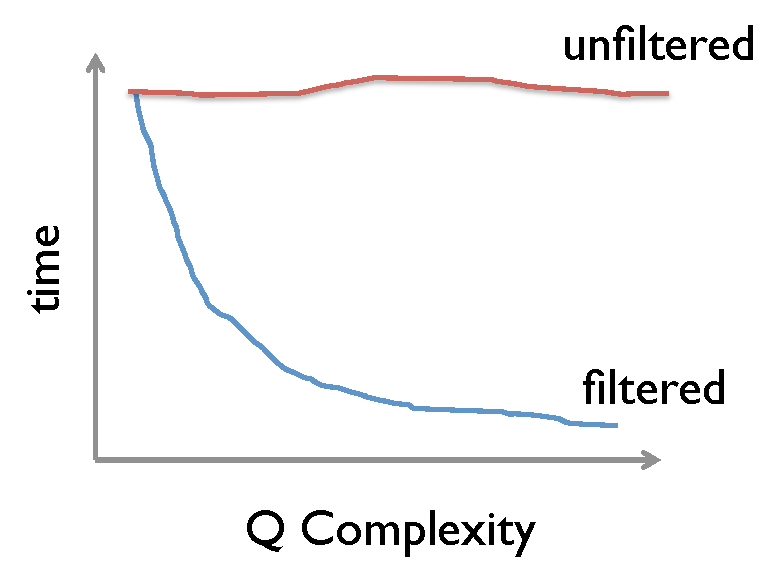
\includegraphics[width = 2in]{figures/complete_qfilter_complexity}
\caption{Varying query complexity.}
\label{f:complete_qfilter_complexity} 
\end{figure}



\subsection{Multi-Query}

Using a previous experimental configuration, we varied the number of queries that are corrupted.  Figures~\ref{}
show the quality and running times of the results for a query log of size 1000 and dbsize of 100k.  
As we can see, the cost increases quadratically with each corrupted query and the accuracy of the proposed fixes increases marginally.  
This is because XXX.

We focus on two scenarios.  {\bf Try multiple corruptions that don't overlap (provenance-wise) with each other}.  This is the condition of multiple silo'd that
corrupt their own logs.  Then {\bf Try multiple corrupted queries where one query modifies the updated state of the other}.  This shows that
it is really hard and hopefully we get close?



To better understand the algorithm, we plot the quality metrics after each fixed query and measure how quickly \sys converges to the final result. 
This suggests that an incremental approach where the user can set a threshold to stop the algorithm may be effective.



\subsection{Real Transactional Workload}

We used the web application workload, and evaluated our alogirthms with artifically injected corruptions.
We compared two types of corruptinos.  In figure~\ref{f:real_existing}, we randomly picked a single existing 
query and corrupted its value.  If the query was an INSERT, we randomly pick a value and perturbed it.
If the transaction was an UPDAET, we randomly varied the SET or WHERE clauses.   We re-ran this
100 times and plot the average and standard deviation of the results.


\section{Discussion}

Systems soluttions would be interesting



\section{Related Work}
\label{s:related}


Scorpion explanation uses data to synthesize predicates that explain.

Why not work.

View construction and query by example.


\balance

% Balancing columns in a ref list is a bit of a pain because you
% either use a hack like flushend or balance, or manually insert
% a column break.  http://www.tex.ac.uk/cgi-bin/texfaq2html?label=balance
% multicols doesn't work because we're already in two-column mode,
% and flushend isn't awesome, so I choose balance.  See this
% for more info: http://cs.brown.edu/system/software/latex/doc/balance.pdf
%
% Note that in a perfect world balance wants to be in the first
% column of the last page.
%
% If balance doesn't work for you, you can remove that and
% hard-code a column break into the bbl file right before you
% submit:
%
% http://stackoverflow.com/questions/2149854/how-to-manually-equalize-columns-
% in-an-ieee-paper-if-using-bibtex
%
% Or, just remove \balance and give up on balancing the last page.
%


\newpage
{
% If you want to use smaller typesetting for the reference list,
% uncomment the following line:
% \small
%\bibliographystyle{acm-sigchi}
\bibliographystyle{abbrv}
\bibliography{main}
}

\techreport{%!TEX root=../main.tex

\appendix



\section{Sometming}

}









\end{document}
